\section{Verification Approach}
%figures : 
We give a basic outline of our proof of our sufficiency theorem.

We want to show that $execute\_tree\_list (tree\_list) \in Error\_States$.

We prove this by first proving the following theorem:
\begin{theorem} \label{etl}
 $execute\_tree\_list (tree\_list) \in circle\_op\_2 (t)$, where $t$ is the last element of $tree\_list$.
\end{theorem}

This is a proof by induction on the size of $tree\_list$.

Our inductive hypothesis is  $execute\_tree\_list (tree\_list') \in circle\_op\_2 (t')$ where $tree\_list'$ is $tree\_list$ with the last element removed and $t'$ is the last element of $tree\_list'$.
We want to show that if our inductive hypothesis holds, then $execute\_tree\_list (tree\_list) \in circle\_op\_2 (t)$.

In order to prove this, we must prove the following lemma:
\begin{lemma} \label{l1}
$execute\_tree\_list (tree\_list') \in circle\_op\_2 (t)$.
\end{lemma}
We prove this directly using $Property 3$ and our inductive hypothesis.

Now, using the fact that $execute\_tree\_list (tree\_list') \in circle\_op\_2 (t)$ (Lemma \ref{l1}),
if $x \in circle\_op\_1(t)$, then  $conc\_ex(x, get\_input (get\_pc (l))) \in circle\_op\_2(t)$,
where $l$ is a leaf of $t$ (Lemma \ref{cop}), and $circle\_op\_2(t) \neq \{\} $ (Property $3'$),
we show that $execute\_tree\_list (tree\_list) \in circle\_op\_2 (t)$.

Now, we can use Theorem \ref{etl} to prove our sufficiency property.
We use the fact that  $execute\_tree\_list (tree\_list) \in circle\_op\_2 (t)$, where $t$ is the last element of $tree\_list$ (Lemma \ref{etl}),
$ circle\_op\_2 (last\_elem (tree\_list)) \cap Error_States \neq empty\_set $ (Property $2$), and 
$circle\_op\_2 (last\_elem (tree\_list)) \subseteq Error\_States $ (Property $2'$)
to show that 
$execute\_tree\_list (tree\_list) \in Error\_States$.


\includegraphics[width=.5\textwidth]{set1.eps}\\
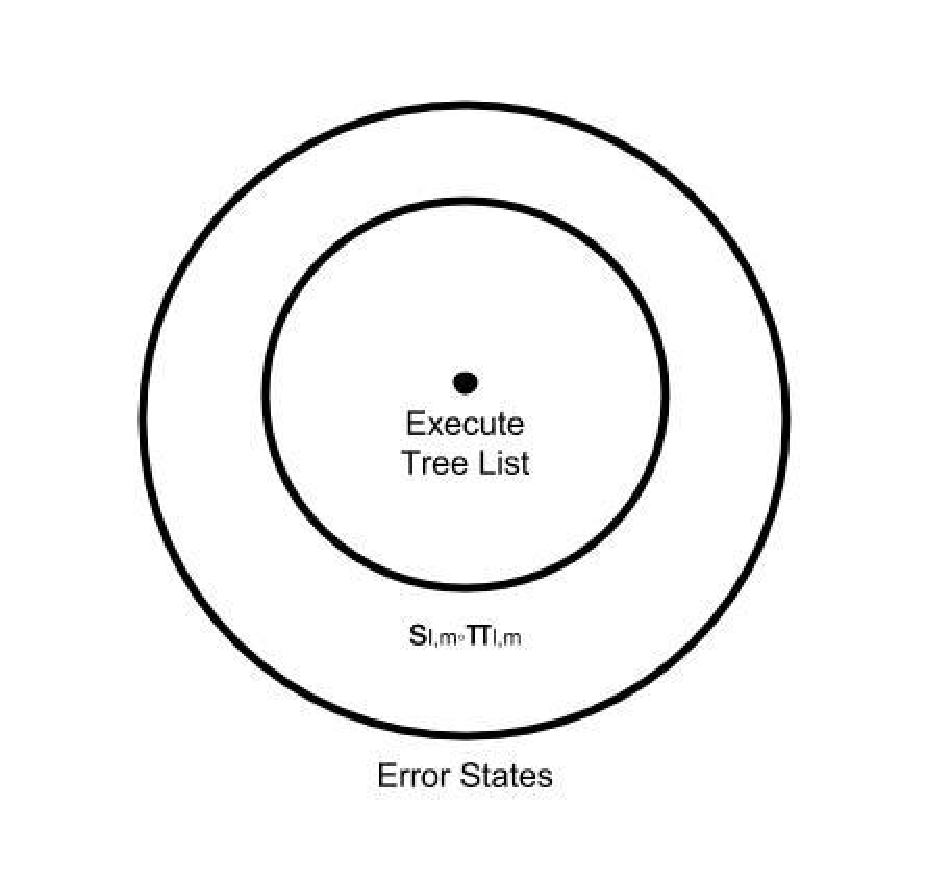
\includegraphics[width=.5\textwidth]{set2.eps}\\
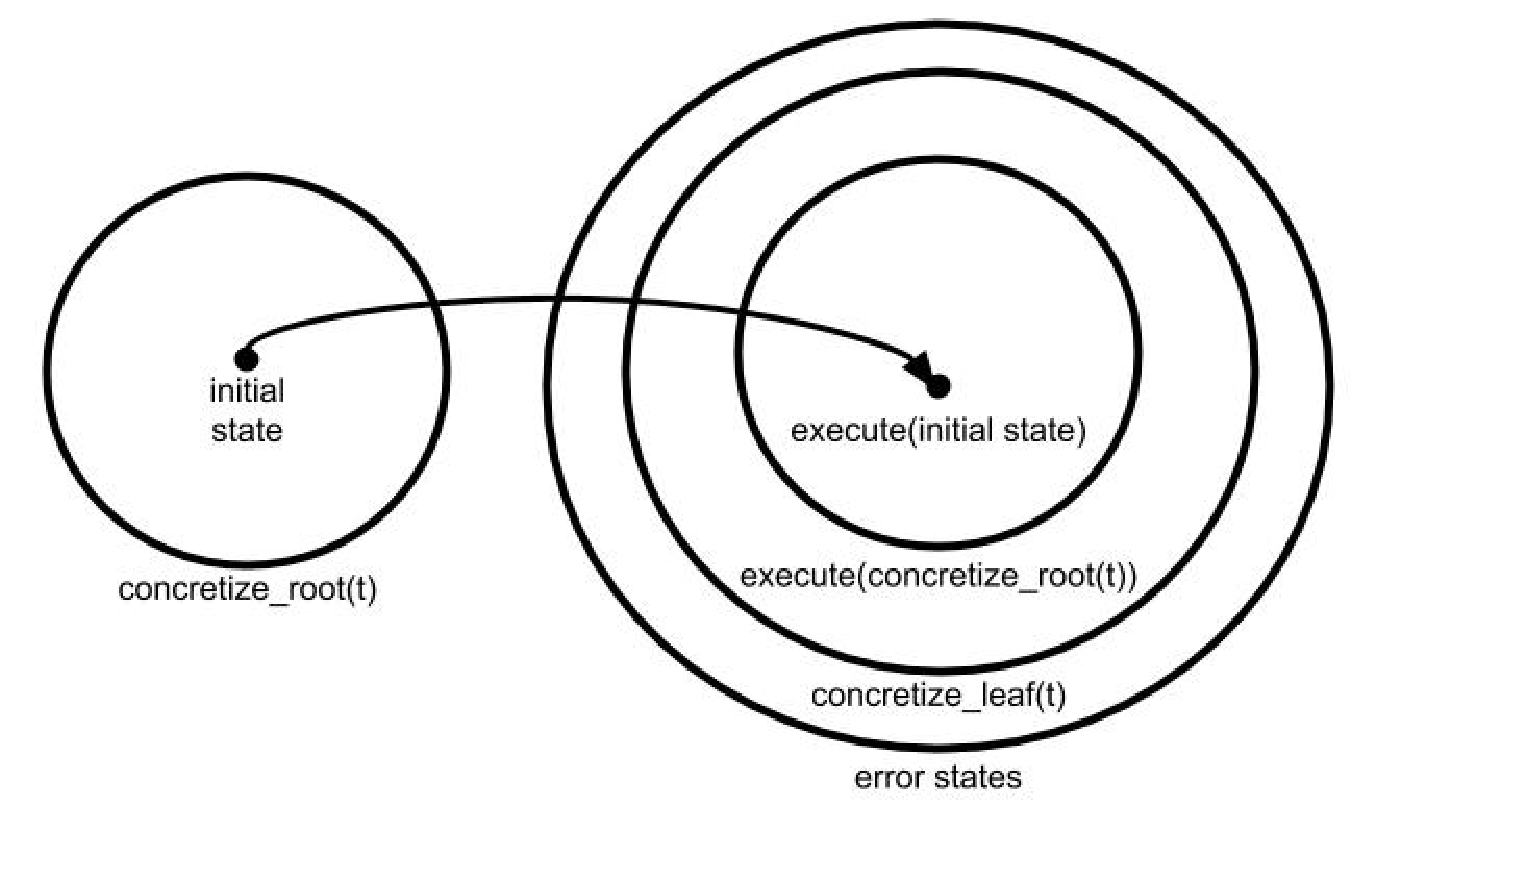
\includegraphics[width=.5\textwidth]{set3.eps}\\
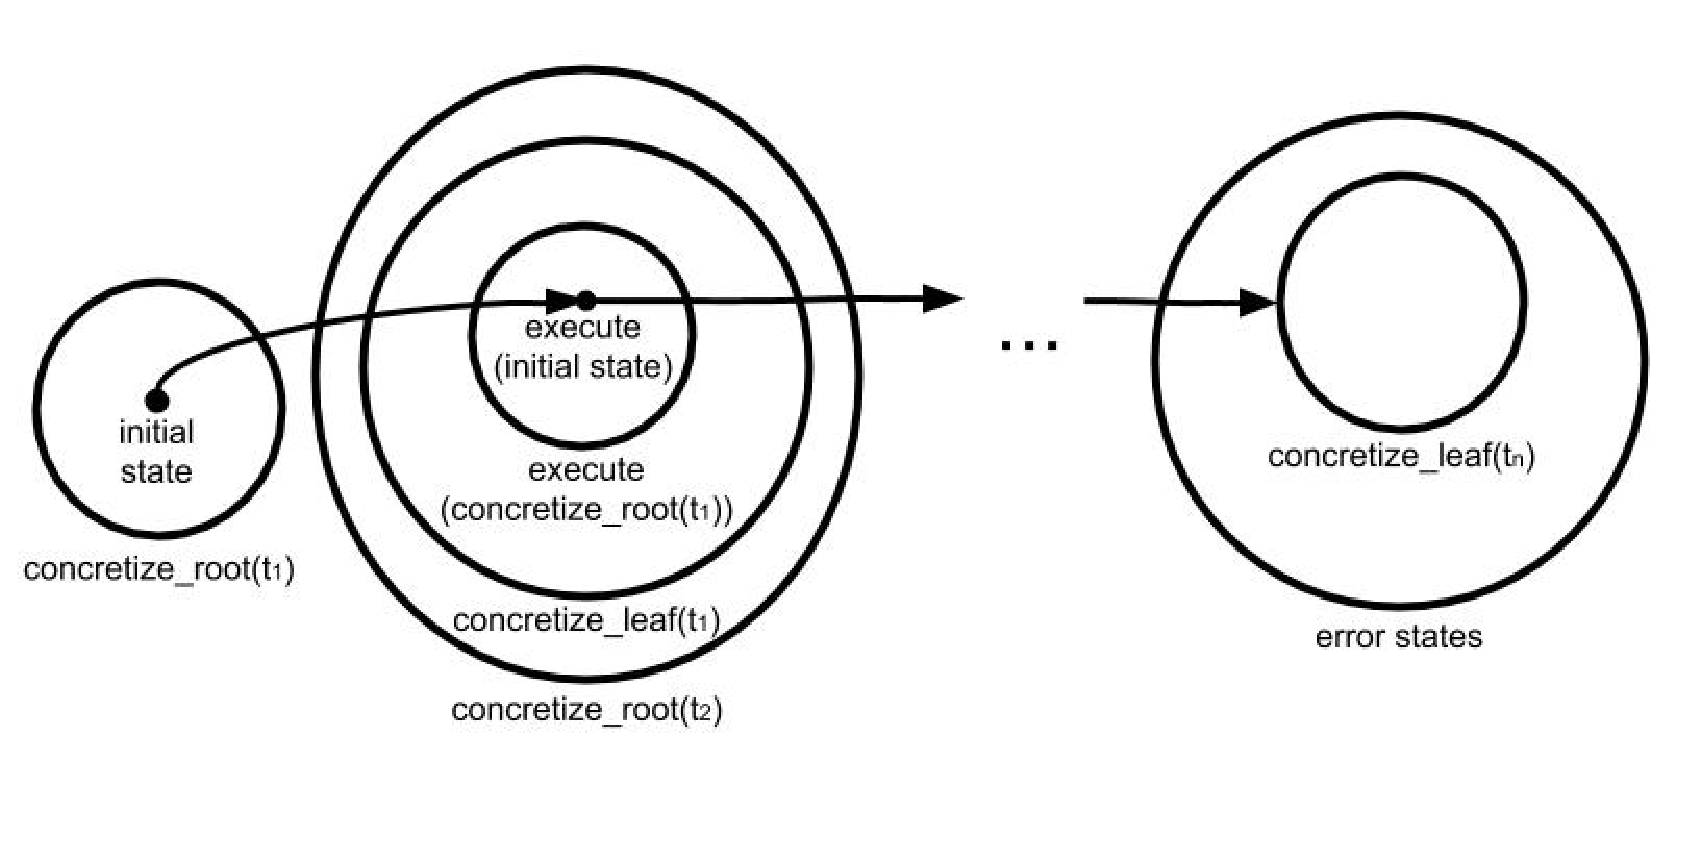
\includegraphics[width=.8\textwidth]{set4.eps}